\documentclass[conference]{IEEEtran}
\IEEEoverridecommandlockouts
\usepackage{graphicx}
\usepackage{algorithm}
\usepackage{algorithmicx}
\usepackage{algpseudocode}
\usepackage[dvipsnames]{xcolor}
\usepackage{amsmath}
\usepackage{hyperref}
\usepackage{caption}
\usepackage{subcaption}
\usepackage{ulem}
\usepackage{tabularx}

% Fix link colors
\hypersetup{
    colorlinks = true,
    linkcolor=red,
    citecolor=red,
    urlcolor=blue,
    linktocpage % so that page numbers are clickable in toc
}

\algblock{Input}{EndInput}
\algnotext{EndInput}
\algblock{Output}{EndOutput}
\algnotext{EndOutput}
\newcommand{\Desc}[2]{\State \makebox[2em][l]{#1}#2}

\newcommand{\tristan}[1]{\color{orange}\textbf{From Tristan:}#1\color{black}}
\newcommand{\english}[1]{\uwave{#1}}

\newcommand{\valerie}[1]{\color{blue}\textbf{From Valerie:}#1\color{black}}


\begin{document}

\title{Simulating the Linux page cache in distributed applications with the WRENCH library}

\author{\IEEEauthorblockN{Hoang-Dung Do$^1$, Val\'erie Hayot-Sasson$^1$, Rafael Ferreira da Silva$^3$, Henri Casanova$^2$, Tristan Glatard$^1$
  }\\
  \IEEEauthorblockA{
    $^1$Department of Computer Science and Software Engineering, Concordia University, Montreal, Canada\\
     $^2$Department of Information and Computer Sciences, University of Hawai‘i at Manoa, USA\\
     $^3$Department of Computer Science, University of Southern California, Los Angeles, USA
  }
}

\maketitle

    \begin{abstract}

        
        The rapid emergence of Big Data seen in recent years has resulted in a 
        growing need for efficient data storing and optimized data analysis techniques. 
        Despite relying on large computing infrastructures with powerful computing capability 
        to process these large datasets, an I/O bottleneck remains. 
        One widely-used approach to minimize the costs of data transfers during
        regular use is through the employment of the page cache.
        While many simulation tools have been developed to 
        support studies in computing systems optimization, page cache simulation 
        has not been fully captured or remains absent from these simulators. 
        The inability to simulate I/O with page cache leads to inaccurate 
        simulations in many situations, especially when dealing with data intensive applications. 
        
        In this paper, we propose a I/O simulation model that characterizes the key features of the page cache.
        We have implemented the model with SimGrid, a simulation framework for 
        distributed systems, using WRENCH, a SimGrid-based workflow simulator. 
        Our simulator is compatible with both single-threaded and multithreaded applications,
        and can simulate both writeback and writethrough cache that can factor into local
        and network-based filesystems.
		
	\end{abstract}		 

	\section{Introduction}
		
        The Linux Page Cache plays an important role in
        the reduction of filesystem data transfer costs. With the page cache, previously
        read data can be reread directly from memory and written data can be written to
        memory before being asynchronously flushed to disk, resulting in improved I/O performance
        on slower storage devices. The performance benefits that can be obtained from using the page
        cache are determined by many factors including the total amount of memory,
        the amount of data being written (i.e. dirty data), and the percentage of available memory available for
        written data. All these factors are important when determining the impact of data transfers on
        application performance, particularly in data intensive applications.

        Characterizing the performance of applications directly on computing infrastructure
        has various shortcomings, which include, limited and shared resources, operational
        costs, unstable environments, and the difficulties in producing reproducible results.
        Simulations address these concerns by providing abstractions for the performance of computer
        hardware, such as CPU, network and storage. Consequently, simulations provide and
        cost-effective, fast, easy and reproducible  way evaluate application performance
        on different infrastructures without having to execute the code.

        The amount of data-intensive applications has been on the rise as a result of
        open-data and data sharing initiatives. Due to the sheer size of the data being
        processed, these applications must be executed on large scale infrastructure
        such as High Performance Computing (HPC) clusters or the cloud. Determining
        which type of infrastructure is the most cost-effective for the particular
        application can be tricky without the help of a simulator.

        Page cache simulation is crucial when simulating data intensive applications,
        which rely on cache hits and writing to memory for additional performance.
        Furthermore, simulating the page cache enables us to study important application-I/O
        bottlenecks which can arise over the course of execution, such as page cache
        starvation~\cite{zhuang2017}.
        While existing simulators can adequately characterize many different computing environments,
        they lack much of the ability to adequately describe the page cache. Some
        simulators try to simulator I/O with page cache, but fail to capture the key features such
        as dirty data and cache eviction policies~\cite{nunez2012simcan,nunez2012icancloud}. 
        Other simulators, such as~\cite{xu2018}, capture the important feature of the
        page cache, but are domain-specific. 

        %However, there is a trade-off between accuracy and scalability, which has been 
        %indicated in some reviews \cite{casanova2014simgrid} \cite{byrne2017review}. 
        %This means that in most cicumstances, users have to, more or less, sacrifice 
        %accuracy for the scalability and performance when their platforms grow to 
        %hundreds or thousands nodes. 

        In this paper, we present WRENCH-Cache, a simulation model of I/O with page
        cache incorporated into WRENCH~\cite{casanova2018wrench}, a workflow management system simulator based on
        the popular SimGrid framework. The goal of WRENCH-Cache is to provide users
        with an accurate representation of a workflow execution, when file system page
        cache is used, while providing a good balance between accuracy and scalability.
        WRENCH-Cache is able to simulate both writeback and writethrough
        cache which would normally be available to local and NFS-based filesystems.
        WRENCH-Cache can provide accurate simulations for large-scale parallel
        applications using the page cache.
         
		
    \section{Related Work}        
    \label{relatedwork}    
        
        \subsection{Page cache}
            
        To improve performance of disk accesses, the page cache was introduced to the Linux kernel. %It contains pages referring to physical pages on disk \cite{linuxdev3rd2010}.
            The goal of the page cache is to try ensure that most I/O operations occur entirely
            within memory space rather than synchronously to and from the storage device.
            All disk-backed data located in the page cache are partitioned into many small pages.
            When a read operation is initiated, the kernel checks whether the required pages are in memory.
            If it is the case, data is read entirely from memory (i.e. \textit{cache hit}). Otherwise,
            the necessary pages must be loaded to memory from the disk (i.e. \textit{cache miss})
            Conversely, for writing, one of three strategies can be applied: direct~I/O (or, ``no-write''),
            writethrough and writeback.
            If direct~I/O is enabled for a given file system, all I/O operations bypass the
            page cache for writes, writing data directly to disk. In contrast, write-through enables the page cache
            for file system writes, but the data is written synchronously from memory to disk. Writeback extends write-through
            by enabling asynchronous writes to disk, meaning that a write call will return once
            the data has been written to memory.
            The writeback strategy is considered to outperform write-through as well as 
            direct I/O as it delays disk writes to perform a bulk write at a later time.
            \cite{linuxdev3rd2010}. 
            

            Cache eviction and flushing strategies are integral to proper page cache functioning.
            Whenever space in memory becomes limited, either as a result of application memory
            or page cache use, page cache data may be evicted. Only data that 
            has been persisted to storage (clean pages) can be flagged for eviction and removed from
            memory. Written data that has not yet been persisted to disk (dirty data) must first
            be copied (flushed) to storage prior to eviction. When sufficient memory is
            being occupied, the flushing process is synchronous. However, even when 
            there is sufficient available memory, written data will be flushed to disk
            at a predefined interval through a process known as \textit{periodical flushing}.
            Periodical flushing only flushes expired dirty pages, which remain dirty in 
            page cache longer than an expiration time configured in the kernel. 
            Different cache eviction algorithms have also been developed and proposed
            \cite{owda2014comparison}.
            The Linux kernel uses a two-list strategy to flag pages for eviction.
            The two-list strategy is based on a least recently used (LRU) policy
            and uses an active and inactive list in its implementation.
            If accessed pages are not in the page cache, they are added to the inactive list. 
            Should pages located on the inactive list be accessed, they will be moved from 
            the inactive to the active list. 
            The lists are also kept balanced by moving pages from the active list
            to the inactive list when the active list grows too large.
            Thus, the active list only contains pages which are accessed more than once 
            and not evictable, while the inactive list includes pages accessed once only, 
            or pages that have be accessed more than once but moved from the active list. 
            Both lists operate using LRU eviction policies meaning the data that has
            not be accessed recently will be moved first.
             
        \subsection{Simulators}
            
            Many simulation frameworks exist to describe the behaviours of applications
            running on the various infrastructures available to users, such as personal computers,
            clouds and clusters.
            These simulators are built with resource models such CPU, network and 
            storage, using various different approaches to describe the hardware.
            For example, there is \textit{CloudSim} and \textit{iCanCloud} for packet-level network models 
            and \textit{DiskSim} the simulates storage hardware functioning.

            Simulators must choose between scalability and accuracy when describing the
            hardware.\cite{casanova2014simgrid}. 
            Fine-grained models allow simulators to achieve high accuracy, 
            but lead to scalability issues due to long simulation time 
            when simulated platforms and applications grow. 
            SimGrid is an open source simulation platform that has been developed 
            not only to balance the trade-off between accuracy and scalability, 
            but also to achieve versatility, allowing the use of the framework 
            to simulate applications in multiple domains. WRENCH, a workflow management
            system simulator based on the SimGrid framework, provides a high-level API
            for simulating workflows, thus facilitating the integration of new models.
            \todo{say more about wrench}
            
            Despite the fact that many sophisticated models for resources have been 
            integrated in simulators, and the page cache shows apparent impacts on I/O
            performance, the simulation model of page cache is still missing in most 
            of simulators.
            For example, SimGrid only simulates I/O operations with storage bandwidths 
            and capacity. 
            SIMCAN is a simulation framework that models page cache by storing data 
            accessed on disk in a block cache \cite{nunez2012simcan}. 
            Page cache is also modeled in the iCanCloud simulator through a component which
            manages memory accesses and cached data \cite{nunez2012icancloud}. However,
            the scalability of the iCanCloud simulator is limited by its sophisticated model.
            Ultimately, none of these simulators provide any writeback cache simulator nor
            cache eviction policys through LRU lists.
            Although cache replacement policies are applied in \cite{xu2018saving} to simulate 
            in-memory caching, their simulator is specific to energy consumption of multi-tier 
            heterogenous networks.
            

            In this study, we use WRENCH 
            to implement our page cache model. We chose WRENCH due to accurate yet scalable implementation, resulting
            from its SimGrid backend, as well as its high-level API.
            We have integrated our model in WRENCH and use the SimGrid API to interact with 
            simulated storage resources.
            This approach allows us to leverage existing features in WRENCH and SimGrid such as process control and synchronization of 
            resource consumption.
            We also leverage the existing SimGrid storage model with capacity 
            and bandwidth properties, which are similar to the characteristics of memory.
            
    \section{Method}
    \label{method}
    In this section, we present our page cache simulation model for file I/O,
    flusing, and eviction. We implement this model in two simulators:
    (1) a standalone Python prototype, and (2) WRENCH-cache, an extension of the WRENCH library.
    We also describe experimental scenarios to evaluate our simulators in various configurations.
     
    We separate our simulation model in two components, the IO
    Controller and the Memory Manager, which together simulate 
    file reads and writes in Linux (Figure~\ref{fig:interaction}). 
    To read or write a file chunk, a simulated application sends a
    request to the IO Controller. The IO Controller interacts as needed with
    the Memory Manager to free memory through flushing or eviction,
    and to read or write to cache. The Memory Manager
    implements these operations, simulates periodical flushing
    and eviction from cache, and reads or writes to disk when necessary.  
    In case write-through strategy is used, IO Controller can also interact directly 
    with disk model to simulate disk writes.
    
    \begin{figure}
           \centering
           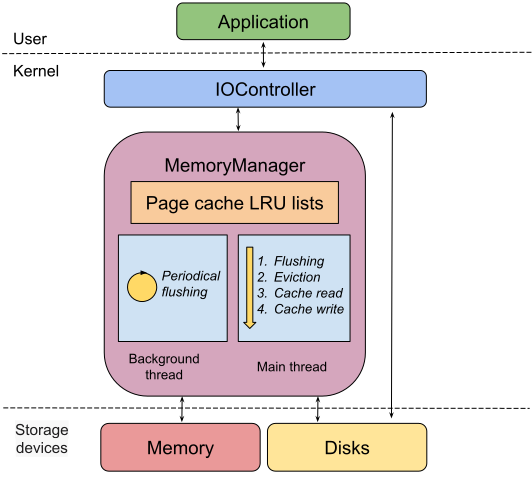
\includegraphics[width=0.85\columnwidth]{figures/interaction.pdf}
           \caption{Overview of the page cache simulator.
           Applications send file read or write requests to the
           IO Controller that orchestrates flushing, eviction, cache
           and disk accesses with the Memory Manager. Concurrent accesses to storage
           devices (memory and disk) are simulated using existing models.}
           \label{fig:interaction}
    \end{figure}

    \subsection{Memory Manager}

    The Memory Manager simulates two parallel threads: the main one
    implements flushing, eviction, and cache I/Os synchronously, whereas
    the second one, operating in the background, periodically searches for
    expired dirty data in page cache LRU lists and flushes them to disk. We
    use existing storage simulation models~\cite{lebre2015} to simulate disk and
    memory, characterized by its storage capacity, read and write
    bandwidths, and latency. Reusing existing storage models allows us to
    simulate bandwidth sharing between concurrent memory accesses and concurrent disk accesses.

    \subsubsection{Page cache LRU lists}

    In the Linux kernel, page cache LRU lists contain file pages. However, 
    due to the large number of file pages, managing lists of pages 
    induces substantial overheads.
    Therefore, we introduce the concept of a data block as a unit to represent data 
    cached in memory. A data block is a subset of file pages stored in
    page cache that were accessed in the same I/O operation. 
    A data block has information about file name, block size, last access 
    time, a dirty flag that represents whether the data is clean (0) 
    or dirty (1), and an entry (creation) time.
    Blocks can have different sizes and a given file can have multiple 
    data blocks in page cache. In addition, a data block can be split into an 
    arbitrary number of smaller blocks.
    \begin{figure}
           \centering
           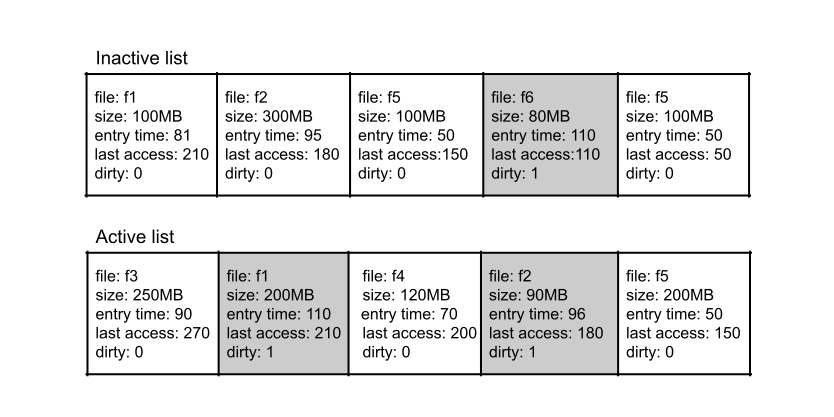
\includegraphics[width=\columnwidth]{figures/lru_lists.pdf}
           \caption{Model of page cache LRU lists with data blocks.}    \label{fig:lrulist}
    \end{figure}    
    
    We model page cache LRU lists as 
    two lists of data blocks, an active list and an inactive list, both ordered by 
    last access time (earliest first, see Figure~\ref{fig:lrulist}).
    As in the kernel, our simulator limits the size of the active list to
    twice the size of the inactive list, by moving least recently 
    used data blocks from the active list to the inactive list~\cite{gorman2004understanding, linuxdev3rd2010}.

    At any given time, a file can be partially cached, completely cached,
    or uncached at all. A cached data block can only reside in one of two 
    page cache LRU lists. The first time they are accessed, blocks are
    added to the inactive list. On subsequent accesses, blocks of the
    inactive list are moved to the top of the active list. Cached blocks 
    written to cache are marked as dirty until they are flushed to disk.

    \subsubsection{Reads and writes}

    Our simulation model supports chunk-by-chunk file accesses
    with a user-defined chunk size. However, for simplicity, we assume that file pages are 
    accessed in a round-robin fashion rather than fully randomly. 
    Therefore, when a file is read, cached data is read only after all uncached data was read, and data from the inactive list is read
    before data from the active list
    (data reads occur from left to right in Figure~\ref{fig:read_order}).
    When a chunk of \emph{uncached} data is read, a new clean block is created 
    and appended to the inactive list. 
    When a chunk of \emph{cached} data is read, one or more existing data blocks in the LRU lists are accessed.
    If these blocks are clean, we merge them together, update the access time and size of the resulting block, 
    and append it to the active list. 
    If the blocks are dirty, we move them independently to the active list, to preserve their entry time. 
    Because the chunk and block sizes may be different, there are situations
    where a block is not entirely read. 
    In this case, the block is split in two smaller blocks and one of them is re-accessed.
    % From Tristan: not sure where to put this nor if it's necessary:
    % , in which chunks are read/written
    % until file is entirely read/written.
    \begin{figure}
           \centering
           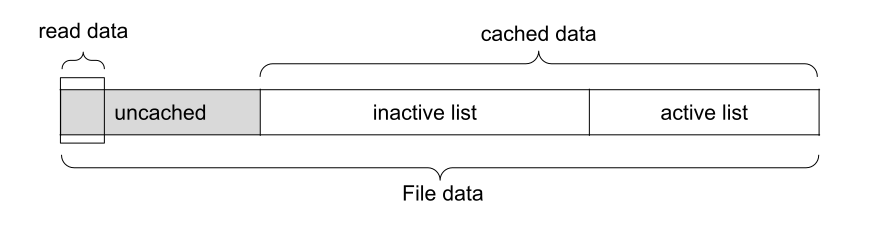
\includegraphics[width=\columnwidth]{figures/read_order.pdf}
           \caption{File data read order. Data is read from left to right: uncached data 
           is read first, followed by data from the inactive list, and finally data from the active list. }
           \label{fig:read_order}
    \end{figure}    

    For file writes, we assume that all data to be written is 
    uncached. Thus, each time a chunk is written, we create a block of dirty data 
    and append it to the inactive list.

    \subsubsection{Flushing and eviction}

    The main simulated thread in the Memory Manager can flush or evict data from the
    memory cache. The data flushing simulation
    function takes the amount of data to flush as parameter. While
    the amount of data to flush is not reached and there are dirty
    blocks remaining in cache, this function traverses the sorted
    inactive list, then the sorted active list, and writes the
    least recently used dirty block to disk, having set its dirty
    flag to 0. In case the amount of data to flush requires that a
    block be partially flushed, the block is split in two blocks,
    one that is flushed and one that remains dirty. Flushing time
    to disk is simulated by the storage model.

    The cache eviction simulation also runs in
    the main thread. It frees up the page cache by traversing and deleting 
    least recently used clean data blocks in the inactive list.
    The amount of data to evict is passed as a parameter and data blocks are deleted 
    from the inactive list until the evicted data reaches the required amount,
    or until there is no clean block left in the list.
    If the last evicted block does not have to be entirely evicted, the block is split in two blocks,
    and only one of them is evicted.
    The cache eviction simulation does not contribute to the simulated time 
    since cache eviction time is negligible in real systems \tristan{a reference would be welcome}.
    
    \begin{algorithm}\caption{Periodical flushing simulation}\label{alg:pdflush}
        \small
        \begin{algorithmic}[1]
            \Input
                \Desc{in}{page cache inactive list}
                \Desc{ac}{page cache active list}
                \Desc{t}{predefined flushing time interval}
                \Desc{exp}{predefined expiration time}
                \Desc{sm}{storage simulation model}
               \EndInput
               \While{host is on}
                \State blocks = expired\_blocks(exp, in) + expired\_blocks(exp, ac) 
                \State flushing\_time = sm.write(blocks)
                \State for blk in blocks: blk.dirty = 0
                \If{flushing\_time $<$ t}
                    \State sleep(t - flushing\_time)
                \EndIf  % Else: do nothing, continue the loop
            \EndWhile
        \end{algorithmic}
    \end{algorithm}

    Periodical flushing is simulated in the Memory Manager
    background thread. As in the Linux kernel, a dirty block
    in our model is considered expired if (1) it is dirty, and (2)
    the duration since its entry time is longer than a
    predefined expiration time. 
    Periodical flushing is simulated as an infinite loop in which 
    the Memory Manager searches and flushes these expired dirty blocks to disk (Algorithm~\ref{alg:pdflush}). 
    % From Tristan: the algorithm is quite straightforward, I don't think this is 
    % necessary
    % In each repetition, Memory Manager finds expired dirty blocks in two 
    % page cache LRU lists (line 8), simulates writes of data of these blocks 
    % to disk (line 9), and mark them as clean (line 10).
    % If the flushing time does not exceed our time interval, the thread is put 
    % to sleep for the remaining time (lines 11-13). 
    % Then based on the state of the host at current simulated time, 
    % the algorithm continues or finishes the loop.
    Because periodical flushing is simulated as a background thread, it can happen concurrently
    with disk I/O initiated by the main thread. This is taken into account by the 
    storage model and reflected in simulated I/O time.

    \subsection{I/O Controller}
     
    \begin{algorithm}\caption{File chunk read simulation of IO Controller}
    \label{alg:read}
        \small
        \begin{algorithmic}[1]
            \Input
                \Desc{cs}{chunk size}
                \Desc{fn}{file name}
                \Desc{fs}{file size (assumed to fit in memory)}
                \Desc{mm}{MemoryManager object}
                \Desc{sm}{storage simulation model}
               \EndInput
               \State disk\_read = min(cs, fs - mm.cached(fn)) \Comment{To be read from disk}
               \State cache\_read = cs - disk\_read \Comment{To be read from cache}
               \State required\_mem = cs + disk\_read
               \State mm.flush(cs + disk\_read - mm.free\_mem - mm.evictable, fn) 
               \State mm.evict(cs + disk\_read - mm.free\_mem, fn) 
               \If {disk\_read $>$ 0}  \Comment{Read uncached data}    
               \State sm.read(disk\_read)  
               \State mm.add\_to\_cache(disk\_read, fn)     
               \EndIf
               \If {cache\_read $>$ 0} \Comment{Read cached}
               \State mm.cache\_read(cache\_read)  
            \EndIf
            \State mm.use\_anonymous\_mem(cs)
        \end{algorithmic}
    \end{algorithm}
    As mentioned previously, our model reads and writes file chunks in a
    round-robin fashion. To read a file chunk, simulated applications send
    chunk read requests to the IO Controller which processes them using
    Algorithm~\ref{alg:read}. First, we calculate the amount of uncached
    data that needs to be read from disk, and the remaining amount is read
    from cache (line 6-7). The amount of memory required to read the chunk
    is calculated, corresponding to a copy of the chunk in anonymous memory
    and a copy of the chunk in cache (line 8). 
    If there is not enough available memory, the Memory Manager is called
    to flush dirty data (line 9). If necessary, flushing is complemented by
    eviction (line 10). Note that, when called with negative arguments, functions
    \texttt{flush} and \texttt{evict} simply return and do not do anything. Then, if there is
    uncached data, memory manager is called to read data from disk and add this 
    data to cache (line 12).
    If cached data needs to be read, the Memory Manager is called to simulate 
    a cache read  and update the corresponding data blocks accordingly (line 15).
    Finally, the memory manager is called to reduce the amount of free memory 
    corresponding to the amount of anonymous memory used by application (line 17).

    \begin{algorithm}\caption{File chunk write simulation of IO Controller}
    \label{alg:write}
        \small
        \begin{algorithmic}[1]
            \Input
                \Desc{cs}{chunk size}
                \Desc{fn}{file name}
                \Desc{mm}{MemoryManager object}
               \EndInput
            \State remain\_dirty = dirty\_ratio * mm.avail\_mem - mm.dirty
            \If {remain\_dirty $>$ 0} \Comment{Write with memory bandwidth}
                \State mm.evict(min(cs, remain\_dirty) - mm.free\_mem)
                \State mem\_amt = min(cs, mm.free\_mem)
                \State mm.write\_to\_cache(fn, mem\_amt) 
            \EndIf
            \State remaining = cs - mem\_amt
            \While {remaining $>$ 0}  \Comment{Write with disk bandwidth}
                \State mm.flush(cs - mem\_amt)
                \State mm.evict(cs - mem\_amt  - mm.free\_mem) 
                \State to\_cache = min(remaining, mm.free\_mem)
                \State mm.write\_to\_cache(fn, to\_cache) 
                \State remaining = remaining - to\_cache
            \EndWhile
            
        \end{algorithmic}
    \end{algorithm}
    Algorithm~\ref{alg:write} describes our simulation of chunk writes in 
    the IO Controller. 
    % Data is written to cache until the amount of dirty data in the cache 
    % exceeds the dirty ratio times the amount of available memory. Data is then written to disk.
    Our algorithm initially checks the  amount of data that 
    can be written as dirty data given the dirty ratio (line 5).
    If this amount is greater than 0, the Memory Manager is requested to evict 
    data from cache if necessary (line 7).
    After eviction, the amount of data that can be written to 
    page cache is calculated (line 8), and a cache write is simulated (line 9). 
    If there is remaining data, this data is written to cache in a loop (line 12 - line 18).
    In this loop, we flush and evict data as possible so that there will be 
    available space for writing (line 13-14).  
    After flushing and eviction, the amount of data that can be written 
    is calculated (line 15) and a cache write is simulated (line 16). 
    We update the remaining amount (line 17) and continue the loop until all data 
    is written.

    In addition to the chunk write simulation with writeback page cache above, 
    we also add a chunk write function with write-through strategy to the IOController.
    This function simply simulates a disk write with the amount of data passed in, 
    then evicts cache if needed and adds this data to cache. 
    
        \subsection{Implementation}

            To validate our simulation model, we created a simple prototype
            simulator independent of existing simulation frameworks and libraries. 
            This allowed us to evaluate the accuracy and correctness of our 
            model in a simple scenario before integrating it to the more complex 
            WRENCH framework. 
            In this prototype we used the following basic storage model for 
            both memory and disk: 
            \begin{align*}
                & t_{r} = D / b_r \\ 
                & t_{w} = D / b_w\
            \end{align*}        
            
            where:
            \begin{itemize}
                \item $t_{r}$ is the data read time
                \item $t_{w}$ is the data write time
                \item $D$ is the amount of data to read or write
                \item $b_r$ is the read bandwidth of the device
                \item $b_w$ is the write bandwidth of the device
            \end{itemize}

            Since bandwidth sharing was not simulated, this prototype does not support
            concurrency: it is limited to single-threaded applications running on systems
            with a single-core CPU. We used this prototype for a first validation of our simulation
            model against a real sequential application running on a real system.
            The source code this prototype is available at
            \url{https://github.com/big-data-lab-team/paper-io-simulation/tree/master/exp/pysim}. We used Python 3.7.

            We also implemented our model in WRENCH, separately from existing WRENCH components. 
            We exposed page cache simulation through a user API, activated using a command-line argument.
            We used SimGrid 3.25 which is available at \url{https://framagit.org/simgrid/simgrid}.
            To implement the simulator, we used the WRENCH 1.6 version at this commit \url{https://github.com/wrench-project/wrench/tree/67185374330d2c4bf274fce222c937e838df5b03}.

\tristan{anything else interesting to mention about the implementation?}

        \subsection{Experiments}

        Our experiments compare real executions with our Python prototype,
        with the original WRENCH, and with our WRENCH-cache extension. We
        evaluate our page cache simulation in single-threaded and
        multi-threaded applications, accessing data on local and remote
        file systems.

        We simulate an application that consists of three single-core, sequential tasks
        where each task reads the file produced by the previous task,
        increments every byte of this file to emulate real processing, and
        writes the resulting data to disk. 
        In real execution, we clear cache before starting the application to make sure 
        the conditions are consistent, the cache is not in use and it is only used by 
        our application.
        In addition, the anonymous memory used by application 
        is released after each task in the pipeline. 
        Thus, we also release the memory used at the end of each task in our simulator.
        We also use a real application
        \textcolor{red}{[Maybe briefly describe this application's purpose
        (e.g. a standard fMRI preprocessing piepeline)]}, to evaluate the
        applicability of our simulation model.

        The real application runs on a dedicated cluster hosted at
        Concordia University, with one login node, 9 compute nodes, and 4
        storage nodes connected with a network bandwidth of 25 Gbps. Each
        compute node has 2 $\times$ 16-core Intel(R) Xeon(R) Gold 6130 CPU
        @ 2.10GHz, 275~GB (256~GiB) \tristan{are you sure it's not 256GB?
        pls check.} of RAM, 6 $\times$ SSDs of 450~GB each with the XFS
        file system, 378~GB of tmpfs, and 126~GB of devtmpfs file system.
        Nodes run CentOS~8.1 with NFS version 4. We use the \texttt{atop}
        and \texttt{collectl} tools to monitor and collect memory status
        and disk throughput.

        To parametrize our simulators, we benchmarked the bandwidths of
        memory, local disk, remote disk (NFS), and network
        (Table~\ref{table:benchmark}). Since WRENCH currently only supports
        symmetrical bandwidths, we use the mean of the read and write
        bandwidth values in our experiments.
            \begin{table}[htbp]
            \centering
            \begin{tabularx}{\columnwidth}{|l
            |>{\centering\arraybackslash}X
            |>{\centering\arraybackslash}X
            |>{\centering\arraybackslash}X|}
            \hline
                Bandwidths  & Cluster (real) & Python simulator & WRENCH simulator\\
            \hline
                Memory read  & 6860    & 4812     & 4812\\
                Memory write & 2764    & 4812 & 4812\\
                Local disk read & 510 & 465 & 465\\
                Local disk write & 420 & 465     & 465\\
                Remote disk read & 515 & - & 445\\
                Remote disk write & 375 & - & 445\\
                Network & 3000 & - & 3000\\
            \hline
            \end{tabularx}
            \caption{Bandwidth benchmarks (MBps) and simulator configurations.
            The bandwidths used in the simulations are the average of the read and write bandwidths
            measured in the cluster.
            Remote disk and network accesses are not simulated in the Python simulator. \tristan{table could be prettified}}
            \label{table:benchmark}
            \end{table}

            As our focus is on I/O rather than compute, we measured
            application task durations on a cluster node and used these
            durations in our simulation. For the Python simulator,
            execution times were directly used in the simulation. For
            WRENCH and WRENCH-cache, we determined the corresponding number
            of flops on a 1~Gflops CPU and used these values in the
            simulation (see Table~\ref{table:cputime}). The final simulated
            platform and application used in our experiment are avaiable at
            \url{https://github.com/wrench-project/wrench/tree/ec6b43561b95977002258c0fe37a4ecad8f1d33f/examples/basic-examples/io-pagecache}.

            \begin{table}[htbp]
            \centering
            \begin{tabularx}{0.8\columnwidth}{|l|>{\centering\arraybackslash}X|}
            \hline
                Input size (GB)  & CPU time (second)\\
            \hline
                3 	 & 4.4 \\
                20  & 28 \\
                50  & 75 \\
                75  & 110 \\
                100  & 155 \\
            \hline
            \end{tabularx}
            \caption{Task CPU time corresponding to input file size.}
            \label{table:cputime}
            \end{table}

            % Finally, because WRENCH simulates applications base on network-communication,
            % we use an infinite bandwidth to eliminate network latency for local I/Os.

            Our first experiment (\textbf{Exp single-threaded}) simply runs one instance of the
            application on a single cluster node, with different input file
            sizes (20~GB, 50~GB, 75~GB, 100~GB), and with all I/Os directed
            to the same local disk. The goal is to validate the simulation model 
            in absence of any concurrent disk access.

            Our second experiment (\textbf{Exp concurrent}) runs concurrent instances of the
            application on a single node, all application instances
            operating on different files of size 3~GB stored in the same
            local disk, sharing the disk bandwidth. We vary the number of
            concurrent application instances from 1 to 32 since cluster
            nodes have 32 CPU cores.

            Our third experiment (\textbf{Exp NFS}) occurs in the same configuration as the
            previous one, albeit reading and writing on a 400-GB NFS-mounted remote disk
            mounted from another compute node. As is commonly
            configured in HPC environments to avoid data loss, in our simulator, 
            NFS client and server read caches are enabled, but there is no cache 
            for writing on client side and server writes are configured with
            write-through cache instead of writeback. 
            Therefore, all the writes happen at disk bandwidth, but
            reads can benefit from cache hits. We simulate write-through by
            writing data directly to disk and adding that data to the server
            cache.

            Finally, we simulate a real application from the neuroimaging
            domain. \textcolor{red}{[Description of the real pipeline with
            nighres (including the workflow engine if it's Dask)]}.
            We simulate this pipeline with simulators using original WRENCH
            and WRENCH-cache. Because our work focuses on I/O time, we
            assume that CPU time is correctly modeled and use the CPU time
            measured in the real pipelines to setup our simulated
            application.

    \section{Results}
    \label{results}

        \subsection{Single-threaded experiment}

        Figure~\ref{fig:single_error} shows the relative error of simulated
        read and write times for the three successive application tasks in \textbf{Exp single-threaded}. The
        page cache simulation model drastically reduces simulation errors
        for all I/O operations except the first read as it involves
        uncached data. Errors are reduced from an average of 345\%
        in the original WRENCH to 46\% in the Python prototype and 39\% in WRENCH-cache.
        Unsurprisingly, the original WRENCH simulator significantly overestimates
        read and write times, due to its lack of page cache simulation
        model.

        Especially, the simulation time errors of \textit{Read 3} with 100 GB of input
        in the simulators with page cache are just under the error in original WRENCH.
        This longer read can be explained with the amount of cached data of files
        at the beginning of the read in reality and simulators shown in
        Fig.~\ref{fig:single_cache}.
        % In this figure, \textit{file $<$i$>$} is the input of \textit{Read $<$i$>$} and
        % output of \textit{Write $<$i-1$>$}.
        With the input size of 20 GB, the amount of cached data of each files after 
        every I/O operation is similar since the page cache can keep all these files.
%             \tristan{what does this refer to?
%             For 20 GB there is still some error in WRENCH-cache, what do you mean 
%``there is no difference in the page cache''?}.
%   Dzung: Some text was lost in a merge, I added it again.
        With the input of 100 GB, the difference between real execution and WRENCH-cache
        simulator can be seen in the amount of \textit{file 3} cache after \textit{Write 2}.
        In real execution, after being written by \textit{Write 2},
        \textit{file 3} is entirely in cache.
        Thus, in \textit{Read 3}, \textit{file 3} is read with memory bandwidth.
        However, in the WRENCH-cache simulator, only a part of \textit{file 3} is
        cached after \textit{Write 2}, which means \textit{Write 2} reads a part of
        \textit{file 3} from disk.
        The reason for the difference is in our WRENCH-cache simulator,
        with 100 GB of input, while \textit{file 3} is being written,
        the page cache is saturated, eviction is then evoked to evict data
        from page cache and make space available for \textit{file 3}.
        However, because the evicted amount is less than required,
        some \textit{file 3} data is evicted after being written, make \textit{file 3}
        partially cached.
        As a result, in \textit{Read 3}, only a part of \textit{file 3} is read from cache
        with memory bandwidth, a part of it is read from disk with disk read bandwidth,
        which is many times slower, leading to longer read time.


            Memory profiling results of real pipeline execution and simulators 
            with 20GB and 100GB input files are illustrated in Fig.~\ref{fig:single_memprof}.
            Because the results with 20Gb, 50GB, 100GB shows a similar pattern,
            we only include the results with 20GB and 100GB in this paper.

            As shown in the figures, the makespans of the simulated pipeline are
            close to the makespan of the real execution with similar patterns of I/O time
            real execution and simulation.
            But more importantly, with all input sizes, similar trends can also be found
            in the lines describing memory status in simulators and the real execution.
            The similar evolutions of amount of cache used (purple lines) in reality
            and simulation show that the use of page cache is well reproduced by the simulators.
            The amount of dirty data (red lines) also follow similar trends,
            which means not only the amount dirty data, but also the flushing and
            periodical flushing mechanisms are accurately modeled in our simulators.
            This can be seen in in the increase of the amount of dirty data during the writes
            and the decrease during the reads and computations.
            According to the results achieved with all input sizes in the experiment,
            we can observe identical trends in reality and simulation with 20GB,
            50GB and 75GB input files. However, with 100GB input file,
            the third read is not correctly simulated, leading to longer simulated time
            than in real execution. This will be explained later in this section.

             Figure~\ref{fig:single_error} shows the relative error of simulated
             read and write times throughout the three application tasks. The
             page cache simulation model drastically reduces simulation errors
             for all I/O operations except the first read that deals with
             uncached data. Errors are reduced from an average of 345\%
             in WRENCH to 46\% in the Python prototype and 39\% in WRENCH-cache.
             The original WRENCH simulator significantly overestimates
             read and write times, due to its lack of page cache simulation
             model.
             Especially, the simulation time errors of \textit{Read 3} with 100 GB of input
             in the simulators with page cache are just under the error in original WRENCH.
             This longer read can be explained with the amount of cached data of files
             at the beginning of the read in reality and simulators shown in
             Fig.~\ref{fig:single_cache}.
             % In this figure, \textit{file $<$i$>$} is the input of \textit{Read $<$i$>$} and
             % output of \textit{Write $<$i-1$>$}.
             With the input size of 20 GB, the amount of cached data of each files after 
             every I/O operation is similar since the page cache can keep all these files.
%             \tristan{what does this refer to?
%             For 20 GB there is still some error in WRENCH-cache, what do you mean 
%``there is no difference in the page cache''?}.
%   Dzung: Some text was lost in a merge, I added it again.
             With the input of 100 GB, the difference between real execution and WRENCH-cache
             simulator can be seen in the amount of \textit{file 3} cache after \textit{Write 2}.
             In real execution, after being written by \textit{Write 2},
             \textit{file 3} is entirely in cache.
             Thus, in \textit{Read 3}, \textit{file 3} is read with memory bandwidth.
             However, in the WRENCH-cache simulator, only a part of \textit{file 3} is
             cached after \textit{Write 2}, which means \textit{Write 2} reads a part of
             \textit{file 3} from disk.
             The reason for the difference is in our WRENCH-cache simulator,
             with 100 GB of input, while \textit{file 3} is being written,
             the page cache is saturated, eviction is then evoked to evict data
             from page cache and make space available for \textit{file 3}.
             However, because the evicted amount is less than required,
             some \textit{file 3} data is evicted after being written, make \textit{file 3}
             partially cached.
             As a result, in \textit{Read 3}, only a part of \textit{file 3} is read from cache
             with memory bandwidth, a part of it is read from disk with disk read bandwidth,
             which is many times slower, leading to longer read time.

            \begin{figure*}
            \centering
            \begin{subfigure}{\linewidth}
                \centering
                   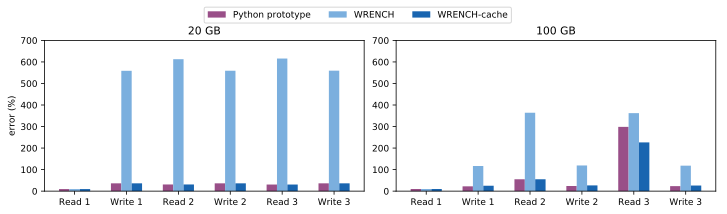
\includegraphics[width=\linewidth]{result/single/figures/single_errors.pdf}
                   \vspace*{-0.7cm}
                   \caption{Simulation errors}
                   \vspace*{0.5cm}
                   \label{fig:single_error}
                \end{subfigure}
            \begin{subfigure}{\linewidth}
                \centering
                %    Gray shades represent task phases (read, compute and write). 
                %    Lines represent memory usage along pipeline execution time.}
                   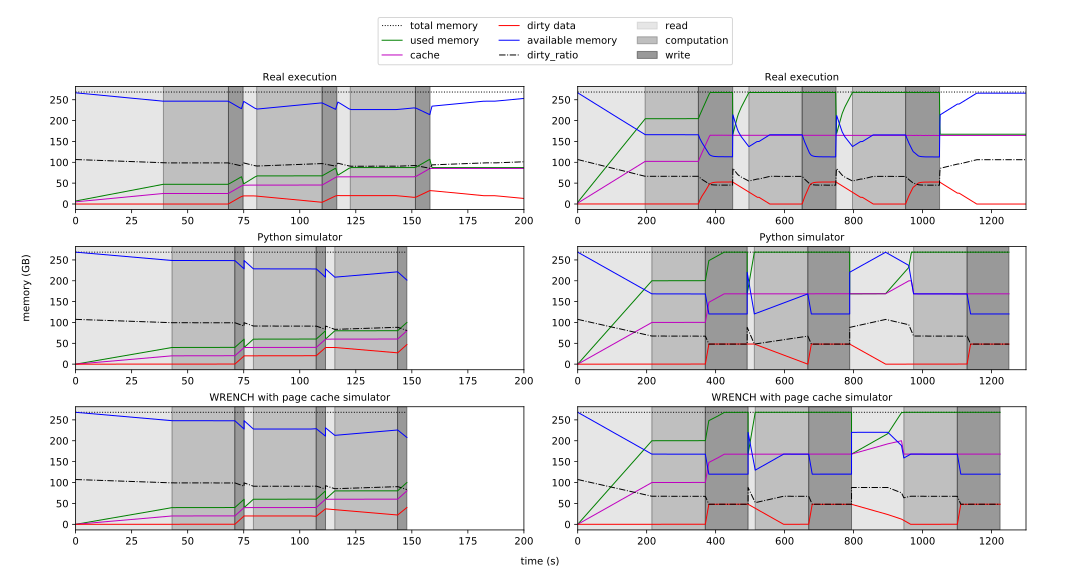
\includegraphics[width=\linewidth]{result/single/figures/single_memprof.pdf}
                   \vspace*{-0.7cm}
                   \caption{Memory profiles}
                   \vspace*{0.5cm}
                   \label{fig:single_memprof}
            \end{subfigure}
            \begin{subfigure}{\linewidth}
                \centering
                   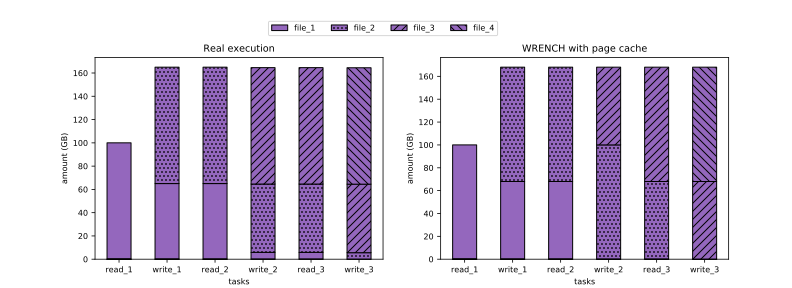
\includegraphics[width=1.05\linewidth]{result/single/figures/cached_files.pdf}
                   \caption{Cache contents}
                %    \textcolor{red}{Update real results of 20GB}}
                   \label{fig:single_cache}
            \end{subfigure}\\
            \caption{Single-threaded results}
            \end{figure*}

            In summary, in this single-threaded experiment, our model can accurately
            simulate I/O time as well as the internal memory behavior.
            This can help confirm that our model is on a right track and
            it can be further improved to achieve higher accuracy.

        \subsection{Multi-threaded experiment}

            \begin{figure*}
            \begin{subfigure}{\linewidth}
                \centering
                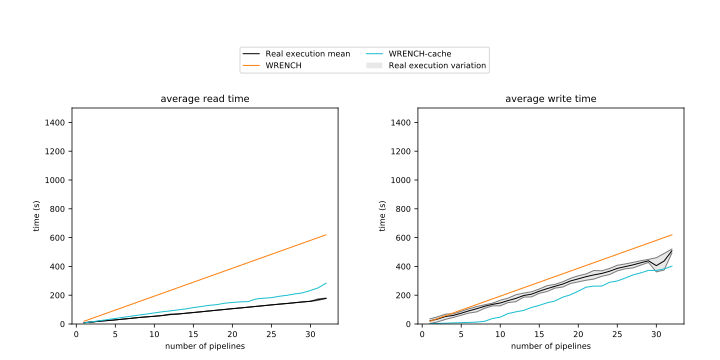
\includegraphics[width=\linewidth]{result/multi/figures/multi_local.pdf}
            \end{subfigure}
            \caption{I/O time of concurrent pipelines with local storage.}
            \label{fig:multi_local}
            \end{figure*}

            In this experiment, we run the real execution in 5 repetitions to
            capture the variability on the cluster.
            The results are analyzed in terms of average I/O time
            of concurrent pipelines shown in Fig.~\ref{fig:multi_local}.

            As is shown in the figure, when the number of pipelines increases,
            the average read time raises accordingly because the amount of data
            increases but memory and disk bandwidths are fixed and shared between pipelines.
            In comparison with original WRENCH, the results from WRENCH-cache are closer
            to reality.
            Especially, when it comes to the average write time,
            although the trend in reality is more complex, our WRENCH-cache
            simulator can still capture the pattern in real execution.
            In both, the average write time gradually increases before surging with the
            same slopes after the number of pipelines reaches 10.
            This can be explained that with less than 10 concurrent pipelines,
            the page cache is not saturated, so all files can be written entirely to
            cache with memory bandwidth in a short time.
            After the page cache is saturated with dirty data (at around
            10 concurrent pipelines in this experiment), this dirty data needs
            to be flushed in order to make space available for writing new data to cache.
            This dirty data is flushed to disk with disk bandwidth, which is much
            slower than memory bandwidth.
            The more pipelines we have, the more data needs to be written, the more data
            needs to be flushed, leading to a sharper increase in the average write time.

            To conclude, the results from WRENCH-cache simulator show that
            our model can also simulate I/O with page cache accurately in a
            multi-threaded application.

        \subsection{Remote storage}

            \begin{figure*}
            \begin{subfigure}{\linewidth}
                \centering
                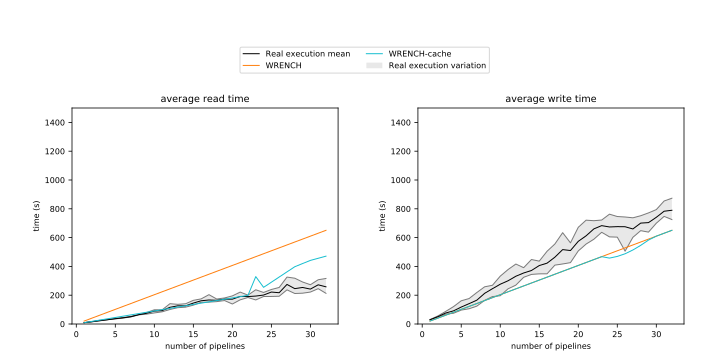
\includegraphics[width=\linewidth]{result/multi/figures/multi_nfs.pdf}
            \end{subfigure}
            \caption{I/O time of concurrent pipelines with NFS}
            \label{fig:multi_nfs}
            \end{figure*}

            Similar to the previous experiment, the real execution with NFS is also
            repeated for 5 times and the results are described with the average I/O time
            shown in Fig.~\ref{fig:multi_nfs}.
            In general, the average I/O time reflect a very similar level of accuracy
            to the previous experiment results when the I/O time of pipelines
            is very close to the real execution.
            The simulated read time if a bit off when the number of pipelines
            surpasses 22, with 264 GB of data in total.
            This is due to the impact of simulated cache eviction when
            the page cache is saturated, which has been seen in
            Fig.~\ref{fig:single_error} with 100 GB of input.
            When it comes to write time, original WRENCH and WRENCH-cache
            results are identical when both are writing directly to disk.

        \subsection{Real application}

    \section{Discussion and Future Work}
    \label{discussion}
        In computing infrastructures, especially those use for data-intensive applications,
        page cache undoubtedly has certain impacts on performance.
        Conducting simulation experiments is an effective approach to predict,
        evaluate the performance of not only application, scheduler but also
        infrastructure settings.
        Unfortunately, page cache is missing in many simulation tools for HPC systems.
        In this study, we proposed a simulation model of I/O with page cache,
        implement it with SimGrid using WRENCH, and evaluate the results
        with different experiments.
        The results shows that our model can result in better simulation accuracy than
        the simulators in which page cache is not modeled.
        Furthermore, this level of accuracy can be achieved without a fine-grained
        level of details.
        This may create opportunities for the model to be applied in simulation of
        big data applications on HPC infrastructures, which leverage memory to
        employ page cache as a disk cache.
        Nevertheless, the model exposed some limitations that can be
        further improved.

        Our short term future work will be re-evaluate the model with asymmetrical
        disk bandwidths that will be released in the next SimGrid version.
        The next step is to study the detail in cache eviction mechanism to make
        the our simulation results closer to reality.
        Another point that needs to be further improved is the ability to configure
        different anonymous memory usage levels of applications since it affects
        the amount of cache used.
        We also plan to support random I/O and file readahead, as well as
        saving and restoring disk state when hosts are turned on/off.

\bibliographystyle{plain}
\bibliography{citation}

\end{document}
